%%%%%%%%%%%%%%%%%%%%%%%%%%%%%%%%%%%%%%%%%%%%%%
% Descripción completa del vehículo
%%%%%%%%%%%%%%%%%%%%%%%%%%%%%%%%%%%%%%%%%%%%%%
\chapter{Componentes del vehículo}
Las características técnicas del vehículo a nivel constructivo se pueden encontrar en la página web del fabricante \cite{Greenland} (\textit{Changzhou Greenland Vehicle Co., Ltd,}) y se muestran en la tabla \ref{Tab:medidas_UALeCARM} para facilitar la labor.

\begin{table}[H]
\caption{Características técnicas del vehículo \textit{UAL-eCARM}.}\label{Tab:medidas_UALeCARM}
\centering
\begin{tabular}{|c |c |c |c|}
\hline % inserts single horizontal line
Parámetro & Medida & Parámetro & Medida \\
\hline
Longitud & 2680 mm  &  Velocidad máxima &  45km/h  \\
\hline
Anchura &  1510 mm  & Autonomía & 90 km \\
\hline
Altura & 1780 mm  & Radio de giro mínimo & 4.3 m \\
\hline
Distancia entre ejes &  1830 mm  & Peso & 740 kg \\
\hline
Paso ruedas traseras & 1285 mm  & Peso sin baterías &  460 kg \\
\hline
Paso ruedas delanteras & 1260 mm  &  Peso máximo &  950 kg \\
\hline
Pendiente máxima &  20\% &  Potencia máxima & 4.3 kW \\
\hline
\end{tabular}
\end{table}

\section{Energía}
La fuente de energía que posee el vehículo son 8 baterías de gel electrolítico de ácido-plomo reguladas por válvula (VRLA) marca Trojan, Figura \ref{fig:Bateria}, \href{https://github.com/ual-arm/ual-ecar-docs/blob/master/Datasheet/TROJAN-6VGEL.pdf}{\textcolor{blue}{datasheet}}. Anteriormente se disponía de 8 baterías de la marca \textit{Greensaver} modelo \textit{SP210-6}, Figura \ref{fig:Bateria-ant}, \href{https://github.com/ual-arm/ual-ecar-docs/blob/master/Datasheet/Greensaver_batteries.pdf}{\textcolor{blue}{datasheet}}. Para acceder a ellas se debe levantar la parte inferior de los asientos del vehículo, Figura \ref{fig:baterias-asientos}. Estas baterías suministran una tensión de 6 Voltios (V) y poseen una capacidad de 189 Amperio-hora (Ah). Con estas características, su conexión se produce en serie obteniendo una tensión total para distribuir en el vehículo de 48V. A pesar de que la tensión suministrada es de 48V, se considera necesario el empleo de conversores DC-DC que suministren líneas de tensión a 5V, 12V y 24V, puesto que no todos los dispositivos electrónicos que incorpora el vehículo trabajan a igual tensión.

Todas los bornes de las baterías se encuentran cableados para realizar la lectura de los niveles de tensión de cada batería. Esta lectura se realiza desde el monitor de baterías desarrollado específicamente para el vehículo descrito en el apartado \ref{Subsec:Monitor_Bateria}. De esta forma se pueden detectar problemas en las baterías de forma individual. Este cableado se muestra en la Figura \ref{fig:baterias-asientos}, los cables rojos son las medidas intermedias. El cable azul de la batería ubicada a la izquierda de la figura representa la conexión de $+48V$ para la electrónica. En la batería ubicada a la derecha de la figura se sitúa el cable negro que proporciona la conexión de referencia. Todas las baterías están sujetas al chasis del vehículo mediante la presión que ejerce un conjunto de tres barras metálicas, con la forma adecuada sujetas al chasis mediante dos varillas metálicas roscadas. Las tuercas que realizan la unión son del calibre \textcolor{red}{xx}. Por otro lado, las tuercas que realizan las conexiones del cableado con las baterías son del calibre \textcolor{red}{xx}.

\begin{figure}[!ht]
\begin{center}
	\subfloat[Trojan 6V-GEL.]{
		\label{fig:Bateria}
		\includegraphics[width=0.35\textwidth]{Figuras/C3-Bateria}}
	\subfloat[Greensaver SP210-6.]{
		\label{fig:Bateria-ant}
		\includegraphics[width=0.4\textwidth]{Figuras/C3-Bateria-ant}}
	\caption{Baterías instaladas en el vehículo.}
\end{center}
\end{figure}

\begin{figure}[!ht]
  \centering
    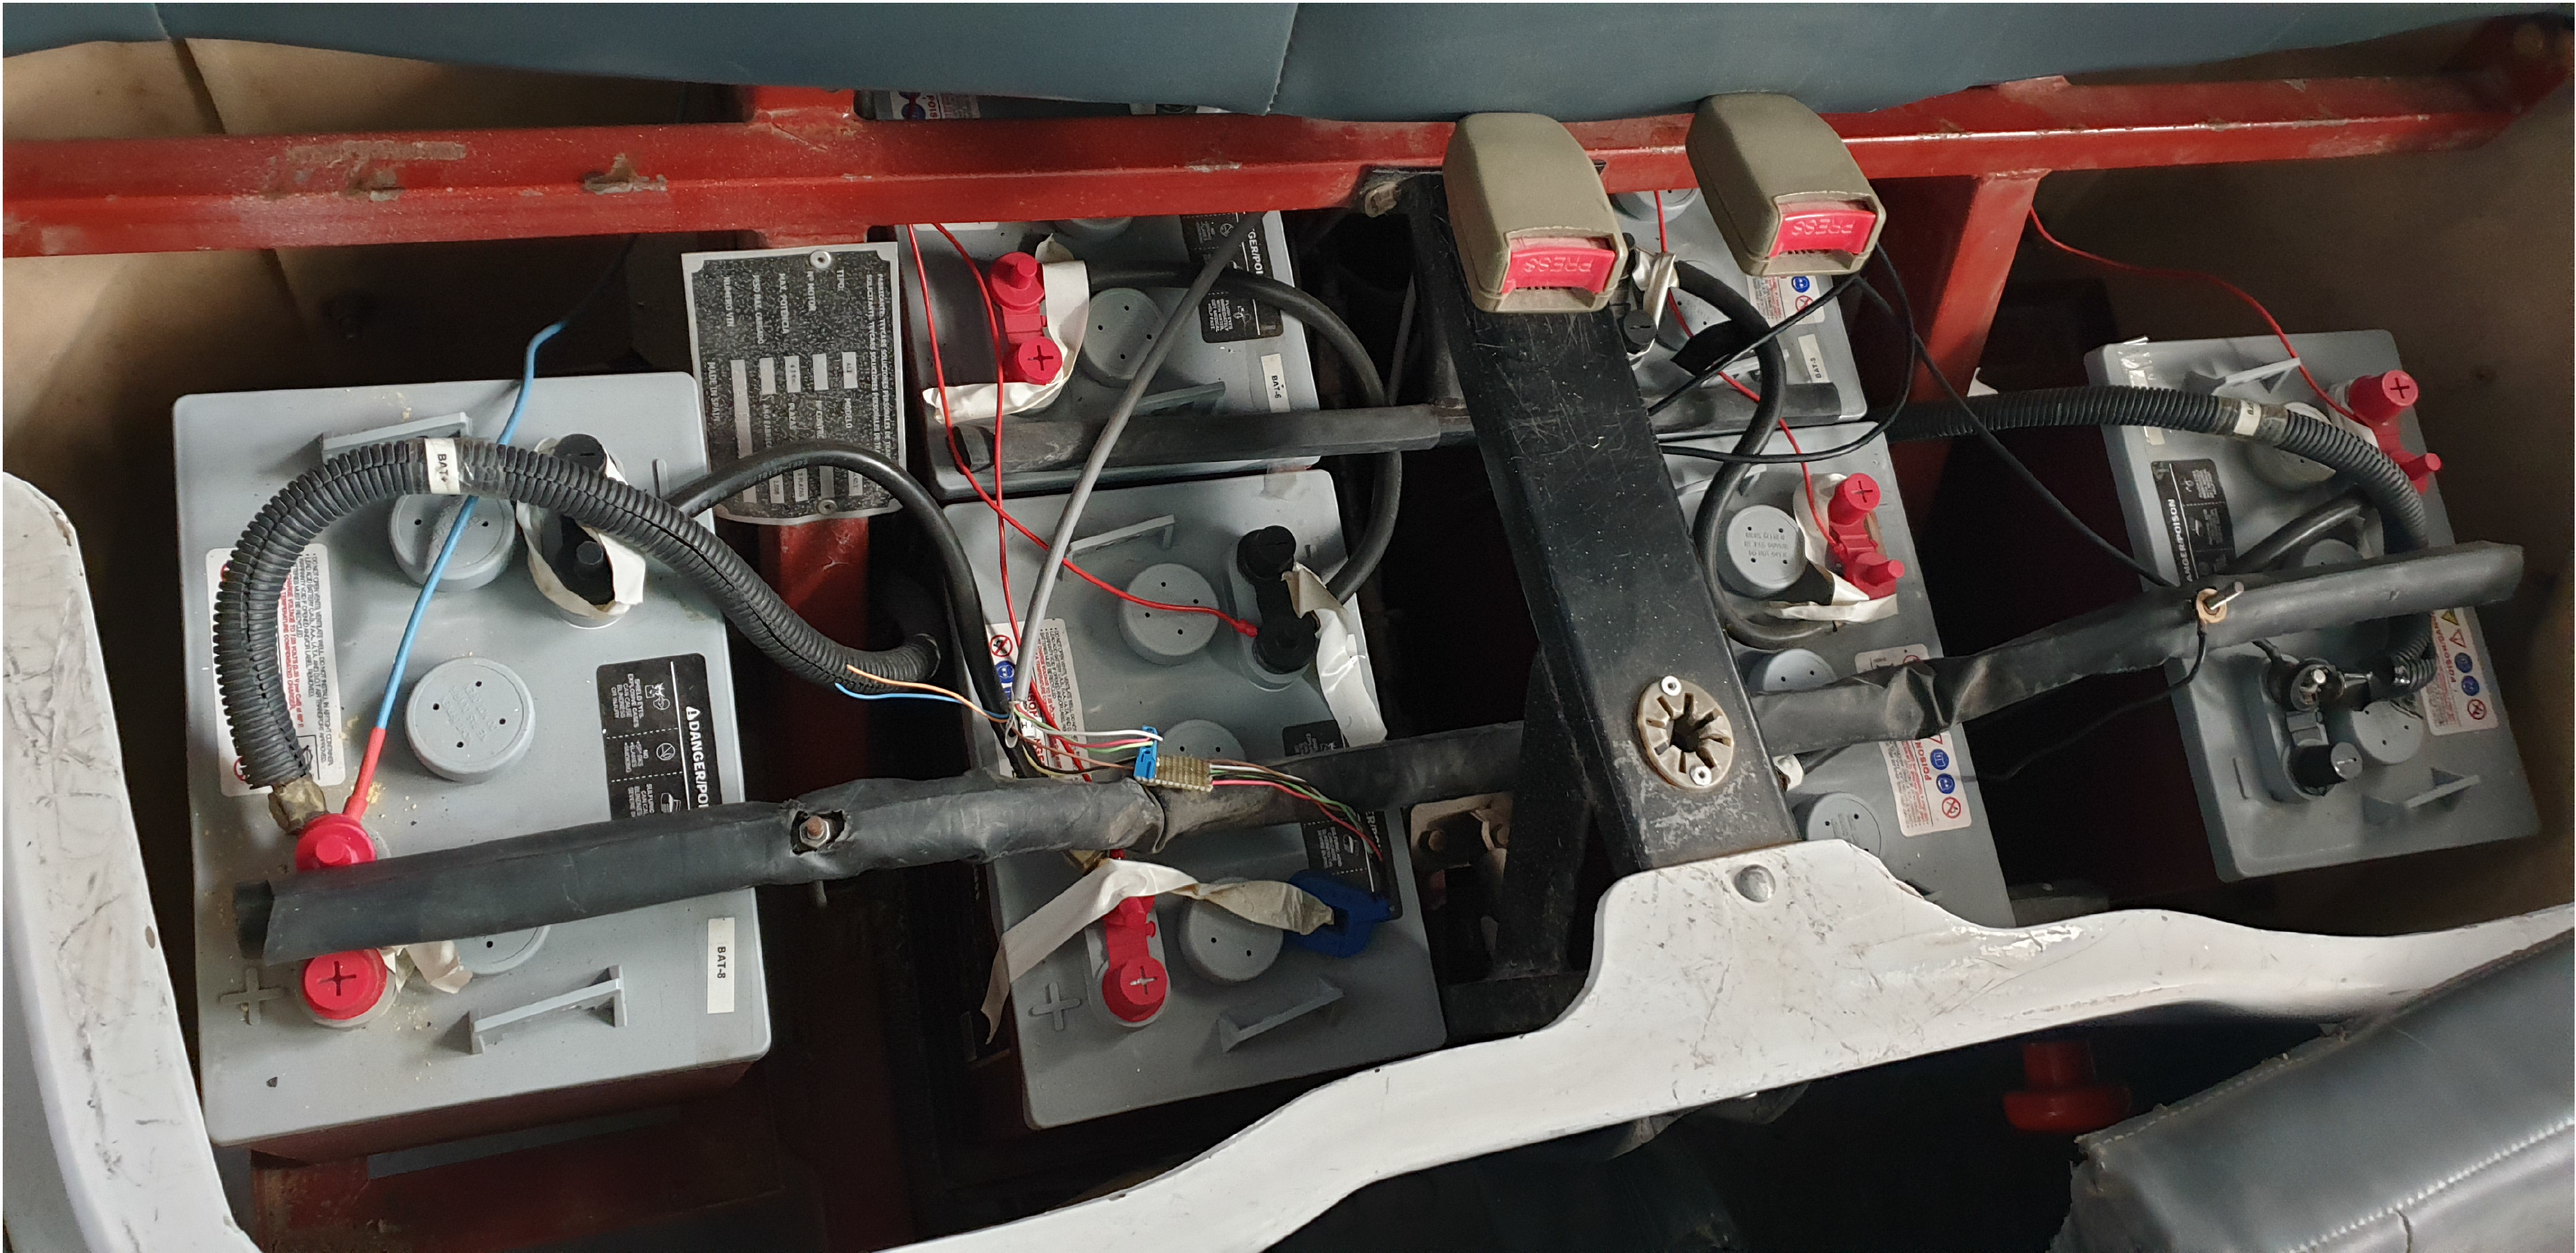
\includegraphics[width=1\textwidth]{Figuras/C3-Baterias-instalacion}
  \caption{Ubicación de las baterías en el vehículo.}
  \label{fig:baterias-asientos}
\end{figure}

\subsection{PowerBox}
Este componente, Figura \ref{fig:PowerBox}, presenta tres funciones principales:
\begin{itemize}
\item Proteger la instalación electrónica mediante la instalación previa de un fusible de 20A.

\item Encender los distintos componentes de forma individual o en pequeñas agrupaciones que permite evitar consumo innecesario de componentes que no se usan.

\item Cortar la alimentación de distintos elementos para manipularlos sin tener que apagar el vehículo entero.
\end{itemize}

A esta caja están conectadas las dos fuentes CC-CC, los dos reguladores y el PC industrial. Como protección principal se emplea un fusible de 20A a la entrada y un display que monitoriza la tensión, intensidad y consumo de todos los componentes conectados. Además se han implementado cinco interruptores que modularizan el encendido de cada componente y uno de ellos actúa como interruptor principal. Esto permite cierto nivel de ahorro energético que se produciría por el encendido de componentes que no se empleen en dicho momento y el encendido de componentes de forma individual para realizar ensayos sobre ellos.  

\subsection{Fuentes de alimentación}
Las baterías, como ya se comentó en la introducción de esta sección, suministran una tensión de 48V, pero no todos los dispositivos requieren dicha tensión. Para el establecimiento de las distintas tensiones requeridas se han empleado dos fuentes CC-CC las cuales convierten de 48V a 12V y 24V respectivamente y dos reguladores conmutados de 5V y 19V respectivamente. 

La fuente CC-CC de 24V, SD-500L-24 mean well, Figura \ref{fig:FuenteDC}, \href{https://github.com/ual-arm/ual-ecar-docs/blob/master/Datasheet/MeanWell_SD-500L-24.pdf}{\textcolor{blue}{datasheet}}, se emplea para la alimentación del motor de la dirección, de los distintos amperímetros de la marca LEM situados por el vehículo (\textcolor{red}{Baterías y} motor) y el sensor láser de la parte frontal. La fuente de 12V, reutilizada de otros proyectos realizados anteriormente, suministra corriente al \textcolor{red}{amperímetro Honeywell que cuantifica la corriente suministrada por las baterías}. El regulador de 5V localizado en la caja denominada \textit{PowerBox} se emplea para la alimentación de aquella electrónica que opera a dicho nivel. El regulador de 19V se requiere para el funcionamiento del monitor situado en la cabina del vehículo. Para su correcto funcionamiento, puesto que el dispositivo integrado abarca un rango de tensiones de salida de 11.85V-22V, se construye un circuito físico para adecuar la tensión a 19V, figura \ref{fig:Regulador}, \href{https://github.com/ual-arm/ual-ecar-docs/blob/master/Datasheet/Regulador-ptn78000h.pdf}{\textcolor{blue}{datasheet}}.

\begin{figure}[!ht]
\begin{center}
	\subfloat[Fuente CC-CC.]{
		\label{fig:FuenteDC}
		\includegraphics[width=0.3\textwidth]{Figuras/C3-DCDC}}
	\subfloat[Regulador.]{
		\label{fig:Regulador}
		\includegraphics[width=0.3\textwidth]{Figuras/C3-Regulador}}
	\subfloat[PowerBox.]{
		\label{fig:PowerBox}
		\includegraphics[width=0.35\textwidth]{Figuras/C3-PowerBox}}
	\caption{Componentes encargados de la administración de corriente.}
\end{center}
\end{figure}

\textbf{HAY QUE AÑADIR UN ESQUEMA QUE MUESTRE EL CABLEADO ELÉCTRICO DE LA ALIMENTACIÓN DEL VEHÍCULO}

\section{Electrónica}
\subsection{Placa microcontrolador Claraquino}\label{Subsec:Claraquino}
Se trata de una placa hardware de código abierto para prototipos con un microcontrolador basado en el ATmega328, depuración mediante JTAG y librería en C para conexión con periféricos comunes y sensores externos (Figura \ref{fig:Claraquino}). La programación y diseño de este dispositivo se encuentra disponible en \href{https://github.com/jlblancoc/claraquino}{\textcolor{blue}{jlblancoc/claraquino}}, su repositorio de Github. En el vehículo actualmente se emplean dos, una para el sistema de dirección y otra para controlar tanto el acelerador como el freno.

\subsection{Monitor de baterías}\label{Subsec:Monitor_Bateria}
Se trata de una placa hardware de código abierto con un microcontrolador ATmega164, depuración JTAG y conversor analógico-digital AD7606 (Figura \ref{fig:Battery_charge}). Su funcionalidad principal es la lectura de los valores de tensión que generan los amperímetros, así como la lectura de la tensión de las baterías. Su programación y el nodo de ROS encargado de su lectura se encuentran disponibles en \href{https://github.com/ual-arm-ros-pkg/ual-ecar-ros-pkg/tree/master/battery_charge}{\textcolor{blue}{ual-arm-ros-pkg/ual-ecar-ros-pkg/battery\_charge}}, proyecto ubicado dentro del repositorio de Github que concentra la mayor parte del código del vehículo, \href{https://github.com/ual-arm-ros-pkg/ual-ecar-ros-pkg}{\textcolor{blue}{ual-arm-ros-pkg/ual-ecar-ros-pkg}}

\begin{figure}[!ht]
\centering
	\subfloat[Claraquino v1.0.]{
		\label{fig:Claraquino}
		\includegraphics[width=0.43\textwidth]{Figuras/C3-claraquino_v1}}
	\subfloat[Monitor de baterías]{
		\label{fig:Battery_charge}
		\includegraphics[width=0.55\textwidth]{Figuras/C3-Monitor_baterias}}
\end{figure}

\subsection{Controlador Curtis}\label{sec:3_Curtis}
Este componente se trata de un controlador Curtis PMC \cite{Controller2012} modelo 1268-5403, Figura \ref{fig:Curtis} con alimentación en el rango comprendido entre 36-48V. \href{https://github.com/ual-arm/ual-ecar-docs/blob/master/Datasheet/Curtis_1268.pdf}{\textcolor{blue}{Manual}}. Su función principal consiste en realizar la etapa de potencia entre la parte electrónica de control y el motor de tracción del vehículo.  

Se trata de un controlador programable, mediante software específico facilitado por el fabricante, basado en un microcontrolador que incluye una sección de potencia MOSFET para un mejor control sobre motores de excitación independiente. Abarca la lectura y actuación sobre gran cantidad de variables lo que permite una variada detección de fallos y un control de gran calidad sobre la velocidad de giro del motor. Su fabricación se lleva a cabo bajo un sistema de gestión de la calidad con la certificación correspondiente según las normas ISO 9001, además de un rango de protección ambiental IP64/IP67.  Tiene una capacidad de hasta 400 amperios/2 minutos para la corriente nominal de la armadura y 50 amperios/2 minutos para la corriente nominal del campo.

\subsection{Relé.}
Se trata de un módulo ya hecho que incluye todos los componentes para que, frente a una señal digital, conmute la salida de un relé. En este trabajo se emplea un módulo que incluye dos relés con una alimentación de 5V. A la salida opera a 48V ya que su función principal es la de conmutar entre la marcha directa y reversa del vehículo. Dicha conmutación no es directa sobre el motor sino que se realiza a través de la unidad de control Curtis mediante las conexiones \textit{J1-10} y \textit{J1-11} del conector lógico \textit{J1} \cite{Controller2012}. El segundo relé se emplea como interruptor de seguridad para evitar que el acelerador lea señales que no genere el sistema de control por interferencias. Esta medida de seguridad se adoptó tras un tiempo en el cual el coche echaba a andar sin causa aparente. 

\subsection{PC Industrial}
Se trata de un PC industrial diseñado especialmente para operar correctamente en ambientes hostiles, Figura \ref{fig:PC_industrial}. Esta condición debe estar presente pues su emplazamiento se encuentra en el maletero del vehículo y cuando se esté trabajando pueden alcanzarse elevadas temperaturas.  

Al PC se encuentran conectados todas las placas de adquisición de datos y las claraquinos que soportan el esquema de control.  Utiliza un sistema operativo Ubuntu Mate 16.04.2 sobre el cual se ha instalado el software \textit{ROS kinetic}.  Dispone de una memoria instalada de 512GB, una memoria RAM de 8GB y un procesador i5 de 3.4GHz y 8 núcleos.

\begin{figure}[!ht]
	\centering
	\subfloat[Controlador Curtis 1268-5403.]{
		\label{fig:Curtis}
		\includegraphics[width=0.3\textwidth]{Figuras/C3-Curtis_Foto}}
	\subfloat[PC Industrial. ]{
		\label{fig:PC_industrial}
		\includegraphics[width=0.35\textwidth]{Figuras/C3-PC_Industrial}}
    \caption{Elementos principales de control del vehículo.}
\end{figure}

\subsection{Codificadores}\label{Subsec:Codificadores}
Para la obtención de la odometría, el vehículo dispone de dos codificadores Phidget IHC3808, Figura \ref{fig:phidget}, instalados en las ruedas traseras. \href{https://github.com/ual-arm/ual-ecar-docs/blob/master/Datasheet/Encoder-Phidget-IHC3808.pdf}{\textcolor{blue}{Datasheet}}. Presentan el límite de escala en 4500 rpm, una resolución de 360 pulsos por revolución y deben ser alimentados en corriente continua a una tensión de 5V. Estos dispositivos se encuentran conectados a una tarjeta LibreDAQ, una plataforma modular de adquisión de datos desarrollada en la Universidad\cite{blanco2015LibreDaq}. El código de esta tarjeta está disponible en el repositorio de Github \href{https://github.com/LibreDAQ/libredaq}{\textcolor{blue}{LibreDAQ/libredaq}}. Esta tarjeta es capaz de leer hasta un máximo de $10^{6}$ pulso/s, por lo que es una plataforma de medida muy sobredimensionada en esta aplicación.

\subsection{Amperímetros}
El vehículo está dotado de tres amperímetros de la marca LEM, dos para la lectura de la corriente en el motor y un tercero para la lectura de corriente que suministran las baterías. Los del motor son del modelo LEM DHR 100, Figura \ref{fig:LEM1}, \href{https://github.com/ual-arm/ual-ecar-docs/blob/master/Datasheet/LEM_DHR_100.pdf}{\textcolor{blue}{datasheet}}. En las baterías, está disponible el sensor modelo LEM HO 240-P-0100, Figura \ref{fig:LEM2}. El único inconveniente de este último dispositivo es que no detecta el sentido de la corriente. Actualmente si se desea determinar la corriente, su módulo si es medido directamente, mientras que el sentido se puede determinar a partir de variables indirectas como el estado de excitación del motor. \textcolor{red}{Hay que calibrar el de las baterías porque genera demasiado ruido y no es posible realizar una medición correcta}.

\begin{figure}[!ht]
\centering
	\subfloat[Phidget IHC3808.]{
		\label{fig:phidget}
		\includegraphics[width=0.3\textwidth]{Figuras/C3-Encoder_rueda.jpg}}
	\subfloat[LEM DHR 100.]{
		\label{fig:LEM1}
		\includegraphics[width=0.3\textwidth]{Figuras/C3-LEM1.jpg}}
	\subfloat[LEM HO 240-P-0100.]{
		\label{fig:LEM2}
		\includegraphics[width=0.3\textwidth]{Figuras/C3-LEM2.jpg}}
	\caption{Sensores instalados en el vehículo e-CARM.}
\end{figure}

\section{Tracción}
\subsection{Motor principal}\label{sec:3_Motor_principal}
El actuador principal del sistema de tracción del vehículo es un motor de impulsión XQ-4.3, figura \ref{fig:motor_eCARM}. Se trata de un motor de excitación en paralelo situado en la parte delantera del vehículo, con clase de aislamiento H y potencia 4.3kW. Se encuentra alimentado a los 48V de las baterías a través del controlador Curtis, el cual controla la excitación, el sentido de la marcha y la velocidad de respuesta del controlador.

\begin{figure}[!ht]
	\centering
		\includegraphics[width=0.5\textwidth]{Figuras/C3-Motor_principal.jpg}{		
		\caption{Motor XQ-4.3.}	
		\label{fig:motor_eCARM}}
\end{figure}

\section{Dirección}
\subsection{Motor dirección} \label{Subsec:Maxon}
Los motores instalados encargados del accionamiento de los mecanismos de la dirección y freno del vehículo, son dos motores de corriente continua, CC, Maxon RE 50 d50mm, escobillas de grafito, 200 Vatios. Este motor tiene una alimentación de 24V y su control físico está regido por la placa \href{https://www.pololu.com/product/1457}{\textcolor{blue}{Pololu High-Power Motor Driver 36v20 CS}}, Figura \ref{fig:Pololu}. Esta placa hace de etapa de potencia entre las señales generadas por la placa Claraquino encargada del sistema correspondiente, transformando la señal PWM y sentido de giro, y en una tensión proporcional a su alimentación. Esta placa incluye, entre otras posibilidades, la posibilidad de medir la corriente consumida por el motor. Además, ambos motores tienen instalados un reductor planetario GP 62 A d62mm, reductora 100:1 y un codificador en cuadratura incremental HEDL5540,500ppv. 3 canales, con line driver RS 422, Figura \ref{fig:Enc_inc}, \href{https://github.com/ual-arm/ual-ecar-docs/blob/master/Datasheet/Encoder_HEDL-5540.pdf}{\textcolor{blue}{datasheet}}.

\subsection{Codificador absoluto} \label{Subsec:Encoder}
Pese a la buena calidad de señal que suministra el codificador incremental acoplado al motor del mecanismo de la dirección, la incertidumbre de la posición absoluta de la dirección supone un problema si el sistema no comienza en el cero del sistema. Como solución a este problema se lleva a cabo el acoplamiento de un codificador absoluto en el tramo en el cual se produce la unión del motor con el mecanismo de la dirección. El acoplamiento se lleva a cabo mediante un mecanismo de transmisión flexible de banda dentada atendiendo a a la sección transversal de la banda. La relación entre el engranaje acoplado al codificador y el acoplado al mecanismo es de 1/3. El codificador empleado se trata del modelo EMS22A del fabricante Bourns, Figura \ref{fig:ENC_dir}, \href{https://github.com/ual-arm/ual-ecar-docs/blob/master/Datasheet/Encoder-EMS22A.pdf}{\textcolor{blue}{datasheet}}. Dicho codificador posee una resolución de 10 bits, una tensión de alimentación de 5V o 3.3V $\pm10\%$ y una corriente máxima de 20mA.\textcolor{red}{Actualmente está averiado. No se realiza la lectura correctamente pese al giro de la transmisión flexible.} En el caso del motor acoplado al mecanismo de frenada, por cuestión de espacio, esta opción para determinar la posición no es viable. Por lo tanto, considerando que el consumo de corriente aumenta conforme se acerca a una posición extrema del mecanismo, se hará que inicialmente el mecanismo se acciones hasta detectar un límite de corriente marcado. Este punto se modelará y la posición será conocida, quedando así establecida la referencia del mecanismo para su respectivo control. \textcolor{red}{Está pendiente realizar la rutina de esta implementación.}

\begin{figure}[!ht]
\centering
	\subfloat[HEDL5540.]{
		\label{fig:Enc_inc}
		\includegraphics[width=0.35\textwidth]{Figuras/C3-Encoder_inc.jpg}}
	\subfloat[EMS22A.]{
		\label{fig:ENC_dir}
		\includegraphics[width=0.2\textwidth]{Figuras/C3-EMS22A}}
		\subfloat[Pololu High-Power Motor Driver 36v20 CS.]{
		\label{fig:Pololu}
		\includegraphics[width=0.25\textwidth]{Figuras/C3-Pololu.jpeg}}
	\caption{Sensores y actuadores acoplados a los motores Maxon.}
\end{figure}

\section{Otros sensores}
También se encuentran instalados otros dispositivos, que no están relacionados de forma directa con este trabajo. El sensor láser SICK Lidar LMS-200, figura \ref{fig:Sick}) situado en la parte frontal del vehículo permite la detección de obstáculos en un radio de alcance de 81m y 180º de visión. El sensor láser Velodyne Lidar Puck, figura \ref{fig:Velodyne}) posee un ángulo de visión de 360º y un alcance de 100m. Este dispositivo consta de 16 rayos y permite la construcción de entornos. También dispone de una cámara estereoscópica y en color del modelo Bumblebee2, figura \ref{fig:Camara}. Esta cámara se encuentra situada en la parte superior del vehículo y está conectada al PC Industrial mediante una conexión firewire.

Para estudios que requieren determinar la posición del vehículo se dispone de un sistema de posición global (GPS) y una Unidad de Medida Inercial (IMU). El GPS, figura \ref{fig:GPS}, se trata del modelo Hemisphere Crescent R100 Series Receiver. La antena receptora se sitúa en la parte superior del vehículo y el receptor en el maletero, conectado al PC a través de un puerto usb. No obstante, este sistema es insuficiente para incluirlo en los lazos de control propuestos en este trabajo por su baja tasa de muestreo, pero es un buen indicador de la posición del vehículo respecto al sistema de referencia geográfico. Finalmente, el IMU antes mencionado, se trata del modelo Xsens MTI 300, figura \ref{fig:IMU}. Este dispositivo posee una frecuencia de muestreo de 10kHz y se conecta al PC mediante USB.

\begin{figure}[!ht]
\centering
	\subfloat[SICK Lidar LMS-200.]{
		\label{fig:Sick}
		\includegraphics[width=0.2\textwidth]{Figuras/C3-sick.png}}
	\subfloat[Velodyne Lidar Puck 16. ]{
		\label{fig:Velodyne}
		\includegraphics[width=0.30\textwidth]{Figuras/C3-velodyne.png}}
	\subfloat[Cámara Bumblebee2.]{
		\label{fig:Camara}
		\includegraphics[width=0.30\textwidth]{Figuras/C3-bumblebee2.png}}
	\\
	\subfloat[IMU Xsens.]{
		\label{fig:IMU}
		\includegraphics[width=0.3\textwidth]{Figuras/C3-Xsens.png}}
	\subfloat[GPS]{
		\label{fig:GPS}
		\includegraphics[width=0.35\textwidth]{Figuras/C3-GPS.jpg}}
	\caption{Sensores instalados en el vehículo.}
\end{figure}

Describir TODO lo que hay instalado en el vehículo. Descripción completa y muy detallada de todos los componentes, características, hojas de fabricantes, que variables generan, si están estandarizadas o no, como se comunican con ROS, ... Incluir comentarios en cursiva con las apreciaciones de los que estén trabajando con ellos, como pequeños trucos o imperfecciones que haya que considerar y aún no se sepa porqué aparecen.

\section{Tareas Pendientes}
Cosas a instalar o calibrar.